\documentclass[]{book}
\usepackage{lmodern}
\usepackage{amssymb,amsmath}
\usepackage{ifxetex,ifluatex}
\usepackage{fixltx2e} % provides \textsubscript
\ifnum 0\ifxetex 1\fi\ifluatex 1\fi=0 % if pdftex
  \usepackage[T1]{fontenc}
  \usepackage[utf8]{inputenc}
\else % if luatex or xelatex
  \ifxetex
    \usepackage{mathspec}
  \else
    \usepackage{fontspec}
  \fi
  \defaultfontfeatures{Ligatures=TeX,Scale=MatchLowercase}
\fi
% use upquote if available, for straight quotes in verbatim environments
\IfFileExists{upquote.sty}{\usepackage{upquote}}{}
% use microtype if available
\IfFileExists{microtype.sty}{%
\usepackage{microtype}
\UseMicrotypeSet[protrusion]{basicmath} % disable protrusion for tt fonts
}{}
\usepackage[margin=1in]{geometry}
\usepackage{hyperref}
\hypersetup{unicode=true,
            pdftitle={Edit This, Please: A Minimal Book Example},
            pdfauthor={Sarah Gaichas, structure from Yihui Xie},
            pdfborder={0 0 0},
            breaklinks=true}
\urlstyle{same}  % don't use monospace font for urls
\usepackage{natbib}
\bibliographystyle{apalike}
\usepackage{color}
\usepackage{fancyvrb}
\newcommand{\VerbBar}{|}
\newcommand{\VERB}{\Verb[commandchars=\\\{\}]}
\DefineVerbatimEnvironment{Highlighting}{Verbatim}{commandchars=\\\{\}}
% Add ',fontsize=\small' for more characters per line
\usepackage{framed}
\definecolor{shadecolor}{RGB}{248,248,248}
\newenvironment{Shaded}{\begin{snugshade}}{\end{snugshade}}
\newcommand{\AlertTok}[1]{\textcolor[rgb]{0.94,0.16,0.16}{#1}}
\newcommand{\AnnotationTok}[1]{\textcolor[rgb]{0.56,0.35,0.01}{\textbf{\textit{#1}}}}
\newcommand{\AttributeTok}[1]{\textcolor[rgb]{0.77,0.63,0.00}{#1}}
\newcommand{\BaseNTok}[1]{\textcolor[rgb]{0.00,0.00,0.81}{#1}}
\newcommand{\BuiltInTok}[1]{#1}
\newcommand{\CharTok}[1]{\textcolor[rgb]{0.31,0.60,0.02}{#1}}
\newcommand{\CommentTok}[1]{\textcolor[rgb]{0.56,0.35,0.01}{\textit{#1}}}
\newcommand{\CommentVarTok}[1]{\textcolor[rgb]{0.56,0.35,0.01}{\textbf{\textit{#1}}}}
\newcommand{\ConstantTok}[1]{\textcolor[rgb]{0.00,0.00,0.00}{#1}}
\newcommand{\ControlFlowTok}[1]{\textcolor[rgb]{0.13,0.29,0.53}{\textbf{#1}}}
\newcommand{\DataTypeTok}[1]{\textcolor[rgb]{0.13,0.29,0.53}{#1}}
\newcommand{\DecValTok}[1]{\textcolor[rgb]{0.00,0.00,0.81}{#1}}
\newcommand{\DocumentationTok}[1]{\textcolor[rgb]{0.56,0.35,0.01}{\textbf{\textit{#1}}}}
\newcommand{\ErrorTok}[1]{\textcolor[rgb]{0.64,0.00,0.00}{\textbf{#1}}}
\newcommand{\ExtensionTok}[1]{#1}
\newcommand{\FloatTok}[1]{\textcolor[rgb]{0.00,0.00,0.81}{#1}}
\newcommand{\FunctionTok}[1]{\textcolor[rgb]{0.00,0.00,0.00}{#1}}
\newcommand{\ImportTok}[1]{#1}
\newcommand{\InformationTok}[1]{\textcolor[rgb]{0.56,0.35,0.01}{\textbf{\textit{#1}}}}
\newcommand{\KeywordTok}[1]{\textcolor[rgb]{0.13,0.29,0.53}{\textbf{#1}}}
\newcommand{\NormalTok}[1]{#1}
\newcommand{\OperatorTok}[1]{\textcolor[rgb]{0.81,0.36,0.00}{\textbf{#1}}}
\newcommand{\OtherTok}[1]{\textcolor[rgb]{0.56,0.35,0.01}{#1}}
\newcommand{\PreprocessorTok}[1]{\textcolor[rgb]{0.56,0.35,0.01}{\textit{#1}}}
\newcommand{\RegionMarkerTok}[1]{#1}
\newcommand{\SpecialCharTok}[1]{\textcolor[rgb]{0.00,0.00,0.00}{#1}}
\newcommand{\SpecialStringTok}[1]{\textcolor[rgb]{0.31,0.60,0.02}{#1}}
\newcommand{\StringTok}[1]{\textcolor[rgb]{0.31,0.60,0.02}{#1}}
\newcommand{\VariableTok}[1]{\textcolor[rgb]{0.00,0.00,0.00}{#1}}
\newcommand{\VerbatimStringTok}[1]{\textcolor[rgb]{0.31,0.60,0.02}{#1}}
\newcommand{\WarningTok}[1]{\textcolor[rgb]{0.56,0.35,0.01}{\textbf{\textit{#1}}}}
\usepackage{longtable,booktabs}
\usepackage{graphicx,grffile}
\makeatletter
\def\maxwidth{\ifdim\Gin@nat@width>\linewidth\linewidth\else\Gin@nat@width\fi}
\def\maxheight{\ifdim\Gin@nat@height>\textheight\textheight\else\Gin@nat@height\fi}
\makeatother
% Scale images if necessary, so that they will not overflow the page
% margins by default, and it is still possible to overwrite the defaults
% using explicit options in \includegraphics[width, height, ...]{}
\setkeys{Gin}{width=\maxwidth,height=\maxheight,keepaspectratio}
\IfFileExists{parskip.sty}{%
\usepackage{parskip}
}{% else
\setlength{\parindent}{0pt}
\setlength{\parskip}{6pt plus 2pt minus 1pt}
}
\setlength{\emergencystretch}{3em}  % prevent overfull lines
\providecommand{\tightlist}{%
  \setlength{\itemsep}{0pt}\setlength{\parskip}{0pt}}
\setcounter{secnumdepth}{5}
% Redefines (sub)paragraphs to behave more like sections
\ifx\paragraph\undefined\else
\let\oldparagraph\paragraph
\renewcommand{\paragraph}[1]{\oldparagraph{#1}\mbox{}}
\fi
\ifx\subparagraph\undefined\else
\let\oldsubparagraph\subparagraph
\renewcommand{\subparagraph}[1]{\oldsubparagraph{#1}\mbox{}}
\fi

%%% Use protect on footnotes to avoid problems with footnotes in titles
\let\rmarkdownfootnote\footnote%
\def\footnote{\protect\rmarkdownfootnote}

%%% Change title format to be more compact
\usepackage{titling}

% Create subtitle command for use in maketitle
\newcommand{\subtitle}[1]{
  \posttitle{
    \begin{center}\large#1\end{center}
    }
}

\setlength{\droptitle}{-2em}

  \title{Edit This, Please: A Minimal Book Example}
    \pretitle{\vspace{\droptitle}\centering\huge}
  \posttitle{\par}
    \author{Sarah Gaichas, structure from Yihui Xie}
    \preauthor{\centering\large\emph}
  \postauthor{\par}
      \predate{\centering\large\emph}
  \postdate{\par}
    \date{2018-08-31}

\usepackage{booktabs}
\usepackage{amsthm}
\makeatletter
\def\thm@space@setup{%
  \thm@preskip=8pt plus 2pt minus 4pt
  \thm@postskip=\thm@preskip
}
\makeatother

\begin{document}
\maketitle

{
\setcounter{tocdepth}{1}
\tableofcontents
}
\hypertarget{prerequisites}{%
\chapter*{Prerequisites}\label{prerequisites}}
\addcontentsline{toc}{chapter}{Prerequisites}

This is a \emph{sample} book written in \textbf{Markdown}. You can use
anything that Pandoc's Markdown supports, e.g., a math equation
\(a^2 + b^2 = c^2\).

The \textbf{bookdown} package can be installed from CRAN or Github:

\begin{Shaded}
\begin{Highlighting}[]
\KeywordTok{install.packages}\NormalTok{(}\StringTok{"bookdown"}\NormalTok{)}
\CommentTok{# or the development version}
\CommentTok{# devtools::install_github("rstudio/bookdown")}
\end{Highlighting}
\end{Shaded}

Remember each Rmd file contains one and only one chapter, and a chapter
is defined by the first-level heading \texttt{\#}.

To compile this example to PDF, you need XeLaTeX. You are recommended to
install TinyTeX (which includes XeLaTeX):
\url{https://yihui.name/tinytex/}.

\hypertarget{intro}{%
\chapter{Introduction}\label{intro}}

You can label chapter and section titles using \texttt{\{\#label\}}
after them, e.g., we can reference Chapter \ref{intro}. If you do not
manually label them, there will be automatic labels anyway, e.g.,
Chapter \ref{methods}.

Figures and tables with captions will be placed in \texttt{figure} and
\texttt{table} environments, respectively.

\begin{Shaded}
\begin{Highlighting}[]
\KeywordTok{par}\NormalTok{(}\DataTypeTok{mar =} \KeywordTok{c}\NormalTok{(}\DecValTok{4}\NormalTok{, }\DecValTok{4}\NormalTok{, }\FloatTok{.1}\NormalTok{, }\FloatTok{.1}\NormalTok{))}
\KeywordTok{plot}\NormalTok{(pressure, }\DataTypeTok{type =} \StringTok{'b'}\NormalTok{, }\DataTypeTok{pch =} \DecValTok{19}\NormalTok{)}
\end{Highlighting}
\end{Shaded}

\begin{figure}

{\centering 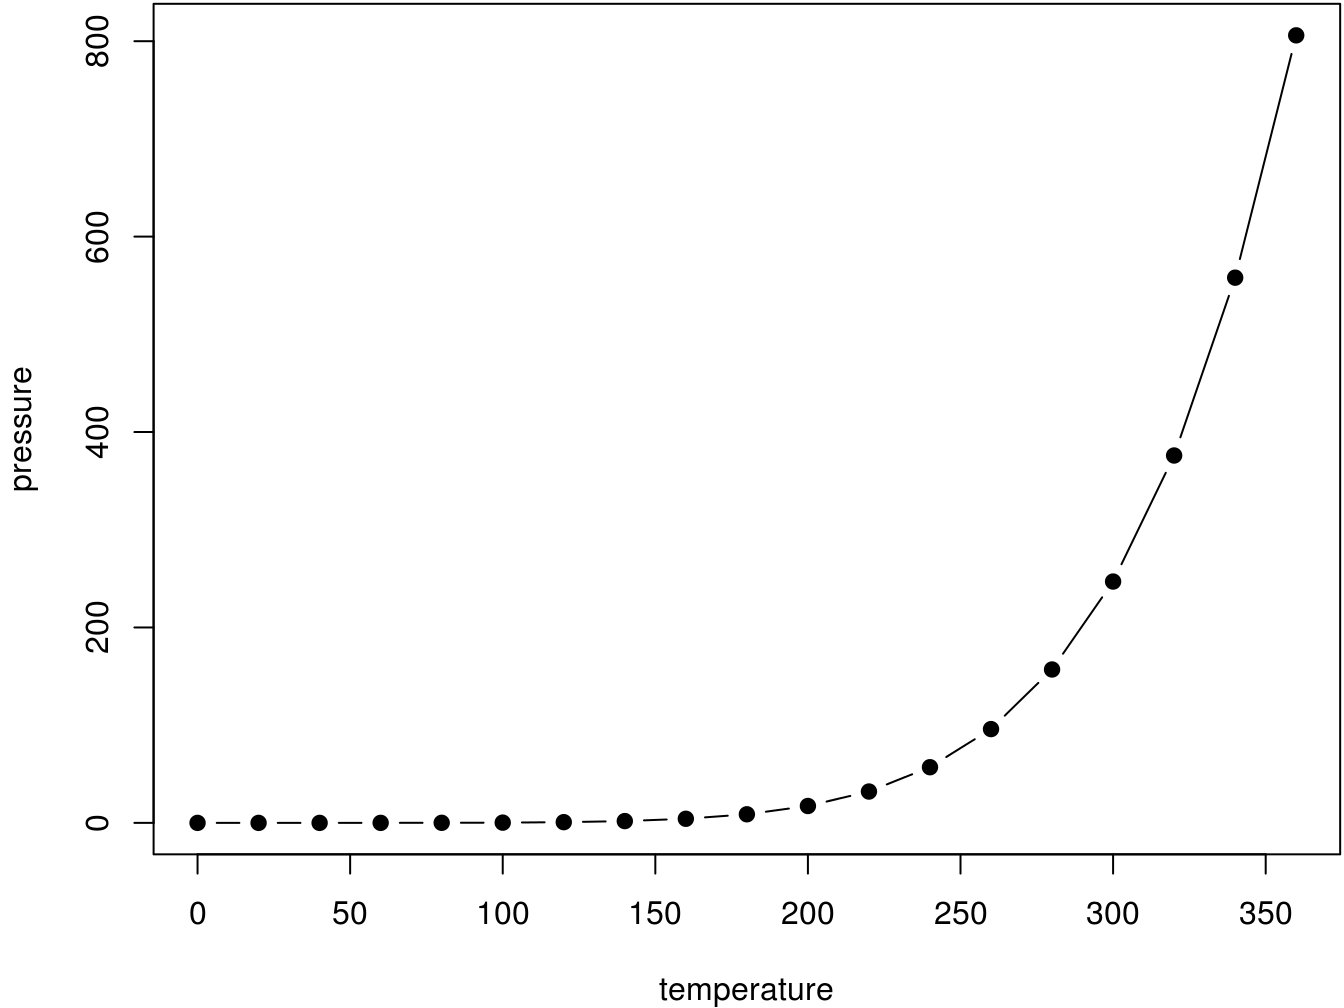
\includegraphics[width=0.8\linewidth]{bookdown-edit-demo_files/figure-latex/nice-fig-1} 

}

\caption{Here is a nice figure!}\label{fig:nice-fig}
\end{figure}

Reference a figure by its code chunk label with the \texttt{fig:}
prefix, e.g., see Figure \ref{fig:nice-fig}. Similarly, you can
reference tables generated from \texttt{knitr::kable()}, e.g., see Table
\ref{tab:nice-tab}.

\begin{Shaded}
\begin{Highlighting}[]
\NormalTok{knitr}\OperatorTok{::}\KeywordTok{kable}\NormalTok{(}
  \KeywordTok{head}\NormalTok{(iris, }\DecValTok{20}\NormalTok{), }\DataTypeTok{caption =} \StringTok{'Here is a nice table!'}\NormalTok{,}
  \DataTypeTok{booktabs =} \OtherTok{TRUE}
\NormalTok{)}
\end{Highlighting}
\end{Shaded}

\begin{table}

\caption{\label{tab:nice-tab}Here is a nice table!}
\centering
\begin{tabular}[t]{rrrrl}
\toprule
Sepal.Length & Sepal.Width & Petal.Length & Petal.Width & Species\\
\midrule
5.1 & 3.5 & 1.4 & 0.2 & setosa\\
4.9 & 3.0 & 1.4 & 0.2 & setosa\\
4.7 & 3.2 & 1.3 & 0.2 & setosa\\
4.6 & 3.1 & 1.5 & 0.2 & setosa\\
5.0 & 3.6 & 1.4 & 0.2 & setosa\\
\addlinespace
5.4 & 3.9 & 1.7 & 0.4 & setosa\\
4.6 & 3.4 & 1.4 & 0.3 & setosa\\
5.0 & 3.4 & 1.5 & 0.2 & setosa\\
4.4 & 2.9 & 1.4 & 0.2 & setosa\\
4.9 & 3.1 & 1.5 & 0.1 & setosa\\
\addlinespace
5.4 & 3.7 & 1.5 & 0.2 & setosa\\
4.8 & 3.4 & 1.6 & 0.2 & setosa\\
4.8 & 3.0 & 1.4 & 0.1 & setosa\\
4.3 & 3.0 & 1.1 & 0.1 & setosa\\
5.8 & 4.0 & 1.2 & 0.2 & setosa\\
\addlinespace
5.7 & 4.4 & 1.5 & 0.4 & setosa\\
5.4 & 3.9 & 1.3 & 0.4 & setosa\\
5.1 & 3.5 & 1.4 & 0.3 & setosa\\
5.7 & 3.8 & 1.7 & 0.3 & setosa\\
5.1 & 3.8 & 1.5 & 0.3 & setosa\\
\bottomrule
\end{tabular}
\end{table}

You can write citations, too. For example, we are using the
\textbf{bookdown} package \citep{R-bookdown} in this sample book, which
was built on top of R Markdown and \textbf{knitr} \citep{xie2015}.

\hypertarget{literature}{%
\chapter{Literature}\label{literature}}

Here is a review of existing methods, directly quoted from
\citep{lewis_method_1903}. Each line from the pdf is a line here; maybe
this makes editing easier? harder?

I REGARD the teaching of English literature and the teaching of
spelling, grammar, and rhetoric as two different professions. It is in
many respects unfortunate that both should have to be practiced by a
single teacher, or a single department, for the best teacher of
literature may be the worst teacher of spelling, grammar, and rhetoric;
but, as our curriculums are at present ordained, we have to face the
situation as best we can. Let us frankly recognize, however, that we are
dealing with two widely different sets of subjects; that the methods
that succeed in the teaching of spelling and grammar may fail utterly
with litera- ture; and that experience gained in one branch cannot be an
infallible guide in the other. My own experience has been almost wholly
in the teaching of literature, and methods of elementary instruction in
that branch will be the subject of this paper. I wish, however, by way
of preface, and in order to avoid a possible misunderstand- ing, to
state briefly an opinion concerning both branches. There is much
complaint against the manner in which kinder- garten ideas have invaded
secondary schools and colleges. I hear it said that we do not discipline
our scholars enough; and that that is why they are growing up
illiterate. Now, my opinion is that, in so far as this complaint relates
to our teaching of spelling, grammar, and rhetoric, it is not without
foundation; I believe that in those subjects some of us do trust too
much to Kindergarten methods-to literary methods; and I am glad to see a
revival of the good old-fashioned discipline. On the other hand, in the
teaching of English literature I think the idea of discipline is already
carried rather too far, and that our schools and colleges would do
better if they employed less of what is commonly called discipline than
they actually do. In this paper I propose to defend what to many will
seem altogether too lax a method; but I wish it distinctly understood
that I am referring only to the teaching of literature, and that, if I
were discussing spelling, grammar, or rhetoric, I should speak very
differently. The first problem that caused me much trouble in my own
experience was as to the degree of minute thoroughness desirable in
reading. The.average student has a very small vocabulary, and, of
course, we want him to extend it. Suppose you are teaching Macbeth. Your
first lesson brings you to Paddock, Graymalkin, kerns, gallowglasses,
Bellona's bridegroom, and a score or more of other expressions that your
student may not know unless he looks them up; and, of course, he will
not look them up unless you make him-that is, unless you devote much of
your time to quizzing the class upon particular words, and insist upon
having everything explained. Of course, the objection to such a plan is
the dryness of the toil involved. Our average student finds it a
positively repellent task, and our object is to make literature attract
him. On the other hand, if you do not make him look up the words he does
not know, will he know Shakespeare at all ? How much of the exquisite
beauty of Romeo, how much of the sublimity of Lear, is wholly lost upon
the student who has not studied Shakes- peare's language. For every
difficulty that you pass over in silence, you will inevitably feel a
sting of conscience, and toward every student with whom you practice the
laxer method you will have moments of feeling yourself a criminal.
Nevertheless, after some years of varied experiments and after much
reflection, I have long since abandoned the stricter method, and for the
last three or four years I have been adding to the burdens of my
conscience about three hundred crimes per annum. It is true that I feel,
after teaching Hamlet, or Lear, or Othello, that none of my students
really know Shakespeare; but, then, who does ? They cannot know him
except in part, and the question for the teacher to decide is: What
part? I have satisfied myself that, so far as my own younger students
are concerned, they will know less about him if they are forced to read
him in what I should call a thorough manner than if they are let off
more easily. In the former case, assuredly not like him; and the
knowledge of Shakespeare possessed by anybody who does not like him must
of necessity be of small value. This seems but a superficial argument;
but there is a deeper principle underlying it. Let us look at the
question in another way. Let us suppose that our chief interest is
merely to increase the student's vocabulary. Even so, I think it might
be plausibly urged that the best way to accomplish this is not by making
him study words. He will enrich his vocabulary more by wide read- ing
than by thorough reading. Consider how we ourselves have learned the
language. I have no idea how large my effective vocabulary is, but I am
certain that not more than I per cent. of it consists of words that I
have looked up. And, moreover, in a matter of this kind, it will not do
to count merely the numbers of words that we know. The quality of our
knowledge is more important to us than the quantity. From dictionaries
and text- books I have learned such words as ``sclerosis,''
``kilogram,'' ``epistemological,'' " isogeotherm," " dicotyledinous." A
friend of mine has recently acquired the word " radiomicrometer," and he
has three times in the last fortnight introduced it casually into
conversation about the weather, with excellent effect. Such words as
these are showy things to wear on the outside, but the part of our
vocabulary that furnishes the really vital garment for our thought is
the integument that grows by nature. Compare with the words that I have
just listed such words as ``father,'' ``mother.'' They afford an extreme
example, for they suggest ideas that are more vitally dear to us than
all the radiomicrome- ters in the world; but in a lower degree I think
all the words that we have unconsciously absorbed, either from the
speech of others or from our own discursive reading, are likewise more
intimately ours than those we have exhumed by a deliberate effort from
dictionaries. I myself, therefore, have discontinued that method of
teach- ing English, because it seemed to me a misguided attempt to find
a short-cut to culture.

\hypertarget{methods}{%
\chapter{Methods}\label{methods}}

We describe our methods in this chapter, quoted directly from
\citep{rowling_harry_2000}, text copied from
\href{http://www.e-bookstoread.com/2017/Harry_Potter_Series_2/index_12.html}{this
site}.

  Harry and Ron had barely finished their third helpings of Christmas
pudding when Hermione ushered them out of the hall to finalize their
plans for the evening.   ``We still need a bit of the people you're
changing into,'' said Hermione matter-of-facdy, as though she were
sending them to the supermarket for laundry detergent. ``And obviously,
it'll be best if you can get something of Crabbe's and Goyle's; they're
Malfoys best friends, he'll tell them anything. And we also need to make
sure the real Crabbe and Goyle can't burst in on us while we're
interrogating him.   ''I've got it all worked out," she went on
smoothly, ignoring Harry's and Ron's stupefied faces. She held up two
plump chocolate cakes. ``I've filled these with a simple Sleeping
Draught. All you have to do is make sure Crabbe and Goyle find them. You
know how greedy they are, they're bound to eat them. Once they're
asleep, pull out a few of their hairs and hide them in a broom closet.''
  Harry and Ron looked incredulously at each other.   ``Hermione, I
don't think -''   ``That could go seriously wrong -''   But Hermione
had a steely glint in her eye not unlike the one Professor McGonagall
sometimes had.   ``The potion will be useless without Crabbe's and
Goyle's hair,'' she said sternly. ``You do want to investigate Malfoy,
don't you?''   ``Oh, all right, all right,'' said Harry. ``But what
about you? Whose hair are you ripping out?''

  ``I've already got mine!'' said Hermione brightly, pulling a tiny
bottle out of her pocket and showing them the single hair inside it.
``Remember Millicent Bulstrode wrestling with me at the Dueling Club?
She left this on my robes when she was trying to strangle me! And she's
gone home for Christmas - so I'll just have to tell the Slytherins I've
decided to come back.''   When Hermione had bustled off to check on
the Polyjuice Potion again, Ron turned to Harry with a doom-laden
expression.   ``Have you ever heard of a plan where so many things
could go wrong?''   But to Harry's and Ron's utter amazement, stage
one of the operation went just as smoothly as Hermione had said. They
lurked in the deserted entrance hall after Christmas tea, waiting for
Crabbe and Goyle who had remained alone at the Slytherin table,
shoveling down fourth helpings of trifle. Harry had perched the
chocolate cakes on the end of the banisters. When they spotted Crabbe
and Goyle coming out of the Great Hall, Harry and Ron hid quickly behind
a suit of armor next to the front door.   ``How thick can you get?''
Ron whispered ecstatically as Crabbe gleefully pointed out the cakes to
Goyle and grabbed them. Grinning stupidly, they stuffed the cakes whole
into their large mouths. For a moment, both of them chewed greedily,
looks of triumph on their faces. Then, without the smallest change of
expression, they both keeled over backward onto the floor.   By far
the hardest part was hiding them in the closet across the hall. Once
they were safely stowed among the buckets and mops, Harry yanked out a
couple of the bristles that covered Goyle's fore head and Ron pulled out
several of Crabbe's hairs. They also stole their shoes, because their
own were far too small for Crabbe- and Goyle-size feet. Then, still
stunned at what they had just done, they sprinted up to Moaning Myrtle's
bathroom.   They could hardly see for the thick black smoke issuing
from the stall in which Hermione was stirring the cauldron. Pulling
their robes up over their faces, Harry and Ron knocked softly on the
door.   ``Hermione?''   They heard the scrape of the lock and
Hermione emerged, shiny- faced and looking anxious. Behind her they
heard the gloop gloop of the bubbling, glutinous potion. Three glass
tumblers stood ready on the toilet seat.   ``Did you get them?''
Hermione asked breathlessly.   Harry showed her Goyle's hair.
  ``Good. And I sneaked these spare robes out of the laundry,''
Hermione said, holding up a small sack. ``You'll need bigger sizes once
you're Crabbe and Goyle.''   The three of them stared into the
cauldron. Close up, the potion looked like thick, dark mud, bubbling
sluggishly.   ``I'm sure I've done everything right,'' said Hermione,
nervously rereading the splotched page of Moste Potente Potions. ``It
looks like the book says it should \ldots{} once we've drunk it, we'll
have exactly an hour before we change back into ourselves.''   ``Now
what?'' Ron whispered.   ``We separate it into three glasses and add
the hairs.''   Hermione ladled large dollops of the potion into each
of the glasses. Then, her hand trembling, she shook Millicent
Bulstrode's hair out of its bottle into the first glass.

  The potion hissed loudly like a boiling kettle and frothed madly. A
second later, it had turned a sick sort of yellow.   ``Urgh - essence
of Millicent Bulstrode,'' said Ron, eyeing it with loathing. ``Bet it
tastes disgusting.''   ``Add yours, then,'' said Hermione.   Harry
dropped Goyle's hair into the middle glass and Ron put Crabbe's into the
last one. Both glasses hissed and frothed: Goyle's turned the khaki
color of a booger, Crabbe's a dark, murky brown.   ``Hang on,'' said
Harry as Ron and Hermione reached for their glasses. ``We'd better not
all drink them in here \ldots{}. Once we turn into Crabbe and Goyle we
won't fit. And Millicent Bulstrode's no pixie.   ''Good thinking,"
said Ron, unlocking the door. ``We'll take separate stalls.''
  Careful not to spill a drop of his Polyjuice Potion, Harry slipped
into the middle stall.   ``Ready?'' he called.   ``Ready,'' came
Ron's and Hermione's voices.   ``One - two - three -''   Pinching
his nose, Harry drank the potion down in two large gulps. It tasted like
overcooked cabbage.

\hypertarget{applications}{%
\chapter{Applications}\label{applications}}

Some \emph{significant} applications are demonstrated in this chapter.

\hypertarget{example-one}{%
\section{Example one}\label{example-one}}

Brutus speaks \citep{mphillips_julius_2017}

It must be by his death. And for my part I know no personal cause to
spurn at him, But for the general. He would be crowned: How that might
change his nature, there's the question. It is the bright day that
brings forth the adder, And that craves wary walking. Crown him that,
And then I grant we put a sting in him That at his will he may do danger
with. Th' abuse of greatness is when it disjoins Remorse from power.
And, to speak truth of Caesar, I have not known when his affections
swayed More than his reason. But 'tis a common proof That lowliness is
young ambition's ladder, Whereto the climber-upward turns his face; But,
when he once attains the upmost round, He then unto the ladder turns his
back, Looks in the clouds, scorning the base degrees By which he did
ascend. So Caesar may. Then, lest he may, prevent. And since the quarrel
Will bear no color for the thing he is, Fashion it thus: that what he
is, augmented, Would run to these and these extremities. And therefore
think him as a serpent's egg, Which, hatched, would, as his kind, grow
mischievous, And kill him in the shell.

\hypertarget{example-two}{%
\section{Example two}\label{example-two}}

{[}Source{]}\url{http://www.elsewhere.org/journal/pomo/1329856939/})

\#\#\#Realism and material posttextual theory

Michel G. Scuglia \emph{Department of Future Studies, University of
Western Topeka} V. Linda Hanfkopf \emph{Department of Literature,
Miskatonic University, Arkham, Mass.}

\hypertarget{contexts-of-absurdity}{%
\subsubsection{Contexts of absurdity}\label{contexts-of-absurdity}}

``Society is part of the genre of culture,'' says Sartre. However,
Lyotard uses the term `the neocapitalist paradigm of narrative' to
denote the failure of cultural art.

The characteristic theme of Werther's{[}1{]} analysis of material
posttextual theory is the difference between society and sexual
identity. If the neocapitalist paradigm of narrative holds, we have to
choose between cultural materialism and neosemiotic textual theory. In a
sense, Debord suggests the use of the neocapitalist paradigm of
narrative to attack and analyse class.

``Sexual identity is fundamentally dead,'' says Baudrillard; however,
according to Tilton{[}2{]} , it is not so much sexual identity that is
fundamentally dead, but rather the futility, and therefore the
meaninglessness, of sexual identity. Wilson{[}3{]} holds that the works
of Smith are postmodern. Thus, many desituationisms concerning a
capitalist reality exist.

In the works of Smith, a predominant concept is the concept of
postpatriarchialist culture. The main theme of the works of Smith is the
dialectic, and subsequent failure, of textual society. Therefore,
Bataille promotes the use of material posttextual theory to challenge
sexism.

If one examines realism, one is faced with a choice: either reject the
neocapitalist paradigm of narrative or conclude that class has objective
value. The subject is interpolated into a subdialectic conceptualist
theory that includes art as a paradox. In a sense, an abundance of
discourses concerning material posttextual theory may be discovered.

The subject is contextualised into a realism that includes culture as a
whole. It could be said that in Dogma, Smith reiterates the
neocapitalist paradigm of narrative; in Mallrats, although, he analyses
realism.

The primary theme of Long's{[}4{]} essay on material posttextual theory
is a mythopoetical totality. Therefore, Sartre uses the term `realism'
to denote the role of the poet as observer.

If material posttextual theory holds, we have to choose between realism
and Batailleist `powerful communication'. But McElwaine{[}5{]} suggests
that the works of Smith are modernistic.

Precultural Marxism holds that narrativity is capable of intentionality,
but only if the premise of material posttextual theory is valid; if that
is not the case, Marx's model of the neocapitalist paradigm of narrative
is one of ``textual discourse'', and hence part of the futility of
truth. However, the main theme of the works of Tarantino is the bridge
between society and sexual identity.

If material posttextual theory holds, we have to choose between the
neocapitalist paradigm of narrative and postdialectic constructivist
theory. Thus, the characteristic theme of Humphrey's{[}6{]} model of
premodern desublimation is a cultural whole.

The subject is interpolated into a neocapitalist paradigm of narrative
that includes narrativity as a totality. Therefore, Sargeant{[}7{]}
suggests that we have to choose between realism and postcapitalist
dialectic theory.

The subject is contextualised into a neotextual paradigm of reality that
includes sexuality as a reality. It could be said that Lyotard suggests
the use of the neocapitalist paradigm of narrative to attack class.

\#\#\#\#. Material posttextual theory and conceptual theory

``Truth is used in the service of hierarchy,'' says Lacan. If realism
holds, we have to choose between material posttextual theory and Marxist
socialism. However, the primary theme of the works of Pynchon is the
common ground between sexual identity and society.

``Consciousness is part of the meaninglessness of art,'' says Debord;
however, according to Reicher{[}8{]} , it is not so much consciousness
that is part of the meaninglessness of art, but rather the rubicon, and
eventually the genre, of consciousness. Neodeconstructivist narrative
implies that class, somewhat paradoxically, has intrinsic meaning. In a
sense, Sartre uses the term `material posttextual theory' to denote the
defining characteristic, and subsequent stasis, of dialectic sexual
identity.

The main theme of Werther's{[}9{]} analysis of conceptual theory is the
difference between class and sexual identity. Thus, Hanfkopf{[}10{]}
states that we have to choose between material posttextual theory and
postsemanticist constructive theory.

A number of discourses concerning the role of the artist as poet exist.
However, Sontag uses the term `conceptual theory' to denote not, in
fact, deappropriation, but predeappropriation.

If substructuralist narrative holds, we have to choose between material
posttextual theory and cultural postsemanticist theory. In a sense,
Debord uses the term `Derridaist reading' to denote the absurdity of
patriarchial class.

\begin{enumerate}
\def\labelenumi{\arabic{enumi}.}
\item
  Werther, M. (1991) The Fatal flaw of Class: Material posttextual
  theory and realism. And/Or Press
\item
  Tilton, E. M. ed. (1988) Realism and material posttextual theory.
  University of Massachusetts Press
\item
  Wilson, A. (1996) The Paradigm of Reality: Socialism, realism and
  subcultural narrative. And/Or Press
\item
  Long, P. R. S. ed. (1989) Material posttextual theory and realism.
  Yale University Press
\item
  McElwaine, K. O. (1971) The Reality of Genre: Realism in the works of
  Tarantino. University of North Carolina Press
\item
  Humphrey, H. ed. (1990) Realism in the works of McLaren. And/Or Press
\item
  Sargeant, W. N. V. (1978) Expressions of Collapse: Realism in the
  works of Pynchon. University of Oregon Press
\item
  Reicher, J. ed. (1981) Realism, socialism and precapitalist
  patriarchial theory. Loompanics
\item
  Werther, S. H. I. (1990) The Broken Door: Realism in the works of
  Joyce. Oxford University Press
\item
  Hanfkopf, F. G. ed. (1974) Realism in the works of Madonna. Loompanics
\end{enumerate}

The essay you have just seen is completely meaningless and was randomly
generated by the Postmodernism Generator. To generate another essay,
follow this link.

The Postmodernism Generator was written by Andrew C. Bulhak using the
Dada Engine, a system for generating random text from recursive
grammars, and modified very slightly by Josh Larios (this version,
anyway. There are others out there).

This installation of the Generator has delivered 18,487,273 essays since
25/Feb/2000 18:43:09 PST, when it became operational.

More detailed technical information may be found in Monash University
Department of Computer Science Technical Report 96/264: ``On the
Simulation of Postmodernism and Mental Debility Using Recursive
Transition Networks``.

More generated texts are linked to from the sidebar to the right.

If you enjoy this, you might also enjoy reading about the Social Text
Affair, where NYU Physics Professor Alan Sokal's brilliant(ly
meaningless) hoax article was accepted by a cultural criticism
publication.

\hypertarget{final-words}{%
\chapter{Final Words}\label{final-words}}

We have finished a nice book.

\bibliography{book.bib,packages.bib}


\end{document}
